\documentclass[
	% -- opções da classe memoir --
	article,			% indica que é um artigo acadêmico
	12pt,				% tamanho da fonte
	oneside,			% para impressão apenas no verso. Oposto a twoside
	a4paper,			% tamanho do papel. 
	]{article}
% ---
% Pacotes
% ---
\usepackage{cmap}				% Mapear caracteres especiais no PDF 
\usepackage{times}			% Usa a fonte Latin Modern
\usepackage[T1]{fontenc}		% Selecao de codigos de fonte.
\usepackage[utf8]{inputenc}		% Codificacao do documento (conversão automática dos acentos)
\usepackage[USenglish]{babel}
\usepackage{indentfirst}		% Indenta o primeiro parágrafo de cada seção.
\usepackage{nomencl} 			% Lista de simbolos
\usepackage{color}				% Controle das cores
\usepackage{color, colortbl}
\usepackage{graphicx}			% Inclusão de gráficos
\usepackage{tabularx}           % in the preamble
\usepackage{amsmath,amssymb}
\usepackage{graphics,graphicx} %linalgjh
\usepackage{multirow}
\usepackage{lscape}
\usepackage{caption,booktabs,array}
\newcommand{\rowgroup}[1]{\hspace{-1em}#1}
\usepackage[flushleft]{threeparttable}
\usepackage{subfigure}
\usepackage{lscape}
\usepackage{rotating}
\usepackage{pdflscape}
\usepackage{comment}
\usepackage{setspace}
\usepackage{subfigure}
\usepackage{geometry}
\usepackage{multicol}
\usepackage{siunitx}
\usepackage{float}
\usepackage{blindtext}
\usepackage{chngcntr} %Para recomecar do 1 a numeracao das tabelas dos anexos
\usepackage{breqn}
\usepackage{microtype}
\hyphenpenalty=10000
\makeatletter% Set distance from top of page to first float
\setlength{\@fptop}{5pt}
\makeatother
\usepackage{float}
\usepackage{hyperref}
	
\definecolor{Gray}{gray}{0.9}
% *****************************************************************
% Estout related commands
% *****************************************************************
\renewcommand{\arraystretch}{1.1}
\newcommand{\sym}[1]{\rlap{#1}}
% \tablefragment: input a Stata-generated table fragment inside a tabular.
% The LaTeX \input opens a group and breaks at the start of an alignment row;
% the TeX primitive \@@input is expansion-safe inside tabulars.
\makeatletter
\newcommand{\tablefragment}[1]{\@@input #1 }
\makeatother
% URL of the shared online appendix (OneDrive). Every mention of the online
% appendix links here; update the address in this single place.
\newcommand{\onlineappendixurl}{https://1drv.ms/b/c/cebd68c6d368de60/IQBJiae2SWdVQbojwq6BhokpAaug9HslTrpD9jVRuiNV5b0?e=Kvc6cU}
\newcommand{\onlineappendix}{\href{\onlineappendixurl}{online appendix}}
\let\estinput=\input% define a new input command so that we can still flatten the document
\newcommand{\estwide}[3]{
  \vspace{0.3cm}{
    \begin{tabular*}
      {\textwidth}{@{\hskip\tabcolsep\extracolsep\fill}l*{#2}{#3}}
      \toprule
      \addlinespace[0.3cm]
      \estinput{#1}
      \bottomrule
      \addlinespace[0.3cm]
    \end{tabular*}
  }
} 
\newcommand{\estauto}[3]{
  \vspace{0.3cm}{
    \begin{tabular}{l*{#2}{#3}}
      \toprule
      \addlinespace[0.3cm]
      \estinput{#1}
      \bottomrule
      \addlinespace[0.3cm]
    \end{tabular}
  }
}

% Allow line breaks with \\ in specialcells
  \newcommand{\specialcell}[2][c]{%
  \begin{tabular}[#1]{@{}c@{}}#2\end{tabular}}

% *****************************************************************
% Custom subcaptions
% *****************************************************************
% Note/Source/Text after Tables
\newcommand{\figtext}[1]{
  \captionsetup{justification=justified,font=footnotesize}
  \caption*{\hspace{0pt}\hangindent=0.0em #1}
}
\newcommand{\fignote}[1]{\figtext{\emph{Note:~}~#1}}
\newcommand{\figsource}[1]{\figtext{\emph{Source:~}~#1}}
% Add significance note with \starnote
\newcommand{\starnote}{\figtext{* p < 0.1, ** p < 0.05, *** p < 0.01. Standard errors in parentheses.}}

% *****************************************************************
% siunitx
% *****************************************************************
\sisetup{
  detect-mode,
  tight-spacing   = true,
  group-digits    = integer,
  input-signs   = ,
  input-symbols   = ( ) [ ] - + *,
  input-open-uncertainty  = ,
  input-close-uncertainty = ,
  table-align-text-post = false,
  input-ignore={,},
  group-separator={,},
  group-minimum-digits=4,
  input-decimal-markers={.}
}
% Primitive input to solve the problem with \toprule inside inputed tables
\makeatletter
\newcommand\primitiveinput[1]
{\@@input #1 }
\makeatother


\geometry{a4paper,tmargin=1in,bmargin=1in,lmargin=1in,rmargin=1in,footskip=55pt}

% ---
% Pacotes de citações
% --- 
\usepackage[round]{natbib}
\bibliographystyle{ecta}
%\usepackage{apacite}

% ---
% Configurações de aparência do PDF final
% alterando o aspecto da cor azul
\definecolor{blue}{RGB}{41,5,195}
% informações do PDF
\makeatletter
\usepackage{hyperref}
\hypersetup{
     	%pagebackref=true,
		colorlinks=true,       		% false: boxed links; true: colored links
    	linkcolor=blue,          	% color of internal links
    	citecolor=blue,        		% color of links to bibliography
    	filecolor=magenta,      		% color of file links
		urlcolor=blue,
		bookmarksdepth=4
}
\makeatother

\tolerance=1
\emergencystretch=\maxdimen
\hyphenpenalty=1000
\hbadness=10000
% --- 

% ---
% compila o indice
% ---
%\makeindex
% ---
% --- 
% Espaçamentos entre linhas e parágrafos 
% --- 
% O tamanho do parágrafo é dado por:
\setlength{\parindent}{0cm}

% Controle do espaçamento entre um parágrafo e outro:
\setlength{\parskip}{6pt}

% Espaçamento entre linhas
\onehalfspacing

\graphicspath{{../Datawork/Output/Figures/}}

\usepackage{titling}

\setlength{\droptitle}{-8em}   % This is your set screw

% ---
% Informações de dados para CAPA e FOLHA DE ROSTO
% ---

\title{Experimental Evaluation of a Financial Education Program in Elementary and Middle School Grades\thanks{\scriptsize Acknowledgements: We would like to thank Cláudia Forte, Alzira Silva, Thiago Nascimento, and Cláudia Donega from the Brazilian Association of Financial Education (AEF-Brasil), José Alexandre Vasco from the Securities and Exchange Commission of Brazil (CVM), and the staff from Municipal Secretariats of Education from Manaus and Joinville. We thank the seminar participants from the Sao Paulo School of Economics at Getulio Vargas Foundation, Insper Institute of Education and Research, the 39th Brazilian Econometrics Society Meeting (SBE), and the 3ie-IFPRI Seminar Series. We also thank Arianna Legovini, Bilal Zia, Miriam Bruhn, Florence Kondylis, and an anonymous referee for their comments and suggestions. Finally, we thank DIME i2i, DEC Research Support Budget, and the Brazil Country Office for funding support. The reproducibility package is available on the GitHub repository \href{https://github.com/vivianamorim/financial-education-brazil/tree/main/Do\%20files}{financial-education-brazil}.}}

\author{Caio Piza\thanks{\scriptsize Development Impact Evaluation Unit (DIME) of the World Bank. Contact: caiopiza@worldbank.org} \and Isabela Furtado\thanks{\scriptsize Insper - Institute of Education and Research. Contact: isabelabf@insper.edu.br} \and Vivian Amorim \thanks{\scriptsize 
 Contact: vivianamorim5@gmail.com}}
\date{}


\begin{document}

\maketitle

\vspace{-50pt}
\noindent\textbf{Abstract}
\vspace{-5pt}

This paper investigates whether providing financial education in elementary and middle school grades improves students' financial proficiency and actual behavior. We use a cluster randomized controlled trial to evaluate a pilot program across 201 Brazilian municipal schools, 101 of which received the intervention in 2015. The findings show positive impacts on financial proficiency (0.07 of a standard deviation), mainly among middle school students, a significant shift in hypothetical attitudes toward saving and consumption, especially among fifth graders, and suggestive evidence of improvements in short-term behavioral outcomes. However, the analysis indicates that the program did not impact students' school achievement up to three years after the intervention, which suggests that its effects were not strong enough to shift students' human capital decisions.

%\noindent Does financial education in elementary and lower secondary school help improve children's intertemporal decision-making process? Evidence on the effectiveness of financial education programs in k-9 public schools in developing countries is scant. We use a randomized controlled trial to test the impacts of a financial education pilot program targeting different elementary and middle school grades. We find positive impacts of the program on financial proficiency and attitudinal and behavioral outcomes. Mediator causal effect analysis suggests that changes in attitudinal and behavioral outcomes are not mechanically mediated by improvements in financial proficiency. Overall, our results indicate that financial education should be made available in the early grades of elementary school.  

\vspace{-5pt}

\noindent\textbf{JEL Codes:} D14, I21, I25, O12, O15


\thispagestyle{empty}
% ---
\pagestyle{plain}

\setcounter{footnote}{0}
\renewcommand{\thefootnote}{\arabic{footnote}}
\setcounter{page}{1}


\section{Introduction} \label{sec:introc1}

Financial literacy is at the center of the education debate. As individuals are increasingly exposed to financial decisions at a young age, the sooner they learn to incorporate the costs of their choices into their decision-making, the better. In fact, the Organization for Economic Cooperation and Development (OECD) recommends that financial education start at school, so that people are educated about financial matters as early as possible in their lives \citep[][Good Practice 9]{OECD2005}.\footnote{In this study, we use financial education and financial literacy interchangeably.} In this context, financial education interventions have been implemented in schools around the world, aiming to develop financial skills that could be conducive to better decision-making throughout individuals' life-cycle \citep{Bruhn2016, berry2018impact, Luhrmann2018, gill2019effects, batty2020experiential, de2021effect, frisancho2023school, bover2026impact}.

Most of the aggregate evidence on the impact of financial education, however, comes from programs aimed at adults, and early results were mixed at best: interventions explained a negligible share of the variance in financial behaviors \citep{Fernandes2014} and modestly improved savings behavior but not loan repayment \citep{Miller2015}. More recently, a meta-analysis pooling 76 randomized controlled trials finds that financial education interventions have a significant impact on financial knowledge (about 0.2 of a standard deviation) and on financial behaviors such as saving, borrowing, and budgeting (about 0.1 of a standard deviation) \citep{kaiser2022financial}.\footnote{The meta-analysis covers more than 160,000 individuals; about three quarters of its treatment-effect estimates come from samples of adults, one fifth from youths aged 14 to 25, and fewer than one tenth from children under 14.}

Financial education might change behavior through at least two channels. The first is financial knowledge itself: financially literate individuals are less likely to make costly financial mistakes, such as high-cost borrowing, and are more likely to take advantage of economic opportunities, such as retirement planning and participation in financial markets \citep{Lusardi2014}. In incentivized convex time budget experiments in Germany, a financial education program made high school students' intertemporal choices more time-consistent, though not more patient \citep{Luhrmann2018}, while, absent any intervention, university students with higher pre-existing financial knowledge made seemingly more patient choices, a pattern attributed to knowledge-driven arbitrage rather than to deeper patience \citep{oberrauch2022cognitive}. Nonetheless, whether gains in financial knowledge drive changes in behavior is rarely tested directly.

The second channel is the shaping of attributes such as self-control and the ability to make forward-looking decisions, particularly in programs aimed at children. Such noncognitive attributes shape schooling decisions and labor market prospects \citep{heckman2006effects, kautz2014fostering, acosta2018role}. In particular, more impatient children and adolescents are less likely to invest in human capital and more likely to consume alcohol, develop obesity, and become pregnant during adolescence, while those with lower self-control are more likely to commit crimes later in life \citep{castillo2011today, sutter2013impatience, golsteyn2014adolescent, moffitt2011gradient}. These attributes are also malleable in childhood: a short classroom program, framed as financial literacy, that had young Turkish students imagine their future selves raised their patience in incentivized choices, an effect still detectable almost three years later, and lowered the incidence of behavioral problems at school \citep{alan2018fostering}; a subsequent arm of the same experiment, targeting grit, increased students' perseverance and school performance \citep{alan2019ever}, as did a nationwide grit curriculum in North Macedonia \citep{santos2021can}. In theory, programs aimed at developing such attributes should be prioritized in childhood, given the expected higher returns per dollar invested \citep{cunha2007technology}.

There is increasing evidence that financial education experiments with high school students are effective in increasing financial literacy, with effects ranging from 0.14 to 0.24 of a standard deviation \citep{bover2026impact, frisancho2023school, Bruhn2016}.\footnote{In a quasi-experiment, \cite{gill2019effects} find evidence that twelfth graders taught financial concepts in U.S. economics classes gained about 13 percentage points on a financial literacy test.} The available literature also points to changes in behavior: treated students save and budget more in a large experiment in Brazilian high schools \citep{Bruhn2016}, and these effects can be long-lasting; nine years after the program, treated students used less expensive credit, defaulted less, and were more likely to own a formal microenterprise \citep{bruhn2025long}. In Peru, seven years after school-based lessons, treated individuals shifted their borrowing toward productive small-business loans on slightly better terms, suggesting credit-financed entrepreneurial activity, although formal business creation is unchanged \citep{frisancho2025lasting}. In Spain, treated students make more patient choices in incentivized tasks months after the course ends \citep{bover2026impact}. Evidence from U.S. state financial education mandates shows that students who were required to take personal finance courses in high school have higher credit scores and fewer delinquencies at ages 18 to 21 \citep{urban2020effects}, finance college through federal student aid rather than costlier private loans \citep{stoddard2020effects}, and rely less on payday loans \citep{harvey2019impact}.

There is also growing evidence on the impacts of financial literacy interventions in elementary and middle school grades.
In an experiment in Belgium, \cite{de2021effect} find that a four-hour online course increased the financial knowledge of eighth and ninth graders by 0.46 of a standard deviation,\footnote{Financial knowledge was measured right after the end of the course.} though without a corresponding change in their consumer choices. \cite{batty2020experiential} find an increase of about 0.25 of a standard deviation in the financial knowledge of fourth graders in an experiment with an experiential ``classroom economy'' program across 20 schools in the United States. \cite{berry2018impact}, on the other hand, do not find impacts on financial literacy in an experiment across 135 Ghanaian elementary and junior high schools, with the programs shifting where children saved rather than raising their total savings. Beyond experiments, \cite{bhattacharya2016effectiveness} find a gain of about 12 percentage points in the financial knowledge of eighth graders attending a voluntary summer program in the United States.

In this paper, we use a cluster-randomized controlled trial to investigate the impact of a financial education pilot implemented in 2015 in elementary and middle school grades in two Brazilian municipalities (Manaus and Joinville). We randomly assigned 101 municipal schools to receive the program, and 100 to a control group. Rather than teaching financial facts alone, the intervention aimed to build the attitudes and everyday competencies behind sound financial choices: telling wants from needs, planning and consuming consciously, saving, and weighing the present against the future consequences of one's decisions. The materials anchor these competencies in everyday situations, with students reading real utility bills, comparing cash and installment prices, budgeting school events, and, in the later grades, making decisions inside stories and games that expose common psychological traps, such as ostentation and immediacy. In short, the program sought to help young students become more conscious of the trade-offs embedded in their daily decisions and more forward-looking. The evaluation focused on grades three, five, seven, and nine for reasons discussed later.

We find positive effects on students' financial knowledge of 0.07 of a standard deviation, on average, driven by the middle school grades (0.1 SD). These magnitudes are below the 0.2 of a standard deviation average for financial knowledge in the meta-analysis discussed above, but that average is dominated by adult samples: among children under 14, the pooled estimates carry 95 percent confidence intervals from 0.01 to 0.55 of a standard deviation for financial knowledge and from 0.02 to 0.11 for financial behaviors \citep{kaiser2022financial}. We also find evidence that the program made students' reported attitudes toward consumption and saving more prudent, particularly fifth graders. Futhermore, for the same age cohort, we find suggestive evidence of changes in some contemporary behavioral outcomes, such as talking about money with parents and friends, indicating linkages to short-term behavioral changes. However, we do not detect robust impacts on contemporary learning outcomes or on medium-term human capital. We use a mediation causal analysis to investigate the potential causal link between gains in financial knowledge and changes in behavioral outcomes. Our results do not point to a compelling causal link between formal knowledge and changes in behavior, consistent with \cite{de2021effect}.

Our paper has four main contributions. First, we document the positive impacts on financial proficiency, attitudes, and behavioral outcomes of a large-scale pilot intervention implemented in elementary and middle school grades.  Second, we show that financial education programs can potentially affect different skills across students' life cycles. Third, we test the overlooked hypothesis that increasing financial proficiency is a necessary condition to change individuals' behavior. Finally, we use student-level data from the Brazilian national standardized exams to assess the program's impacts on students' contemporary and medium-term human capital.

Apart from this introduction, this paper is organized as follows. Section \ref{sec:pilot} describes the pilot program and its implementation. Section \ref{sec:data_c} describes the data collection. Section \ref{sec:identification} introduces the empirical strategy, whereas Section \ref{sec:results} discusses the results. We then conclude.


\newpage
\section{Financial Education Pilot in Elementary and Middle Schools}\label{sec:pilot}

The National Strategy for Financial Education (\textit{Estratégia Nacional de Educação Financeira} -- ENEF) was established by the Brazilian Federal Government in 2010 to promote financial education and empower individuals to make autonomous financial decisions.\footnote{ENEF was instituted by Federal Decree 7.397 of December 22, 2010. It brings together the Ministry of Education, the Central Bank of Brazil, the Securities and Exchange Commission of Brazil (CVM), the Ministry of Finance, the Superintendence of Private Insurance (SUSEP), and the Superintendence of Complementary Pension (PREVIC).} Between August 2010 and December 2011, ENEF implemented a pilot financial education program in public high schools across six states -- São Paulo, Rio de Janeiro, Ceará, Tocantins, Minas Gerais, and the Federal District. The program's impact was assessed through a randomized controlled trial involving 891 schools and approximately 20,000 students, and generated significant improvements in students' financial knowledge, saving intentions, financial autonomy, and participation in household financial decisions \citep{Bruhn2016}. Building on these results, in 2014 ENEF commissioned the Brazilian National Committee on Financial Education (\textit{Comitê Nacional de Educação Financeira} -- CONEF) to extend the program to elementary and middle school grades. The pilot of this new program is the object of our evaluation.

The pilot was implemented during the 2015 school year in municipal schools of Joinville and Manaus, whose respective Municipal Secretariats of Education voluntarily joined the initiative. The two cities represent distinct socioeconomic contexts: Manaus, the capital of Amazonas, lies in the northern part of the country, while Joinville, a municipality of Santa Catarina, is located in the more affluent South. By 2016, Joinville exhibited higher per capita income (USD 14,000 vs.~USD 11,000), a higher Municipal Human Development Index (0.809 vs.~0.737), higher school attendance rates among 6- to 14-year-olds (97\% vs.~94\%), and stronger performance on the Brazilian Education Development Index (IDEB) at both elementary and middle school levels. While these differences introduce regional variation in the environment in which the program was delivered, they also extend the external validity of our findings to two economic and educational contexts that are representative of much of Brazil's public-school network.

\subsection{Teaching Materials}\label{subsec:materials}

The program rests on a pair of teaching collections published in 2014 by CONEF -- a student book (\textit{Livro do Aluno}) and a teacher book (\textit{Livro do Professor}), with one volume per grade from the 1\textsuperscript{st} to the 9\textsuperscript{th} year, totaling 18 volumes.\footnote{The materials are publicly available through the ENEF portal and were coordinated editorially by the Brazilian stock exchange (BM\&FBOVESPA, now B3). They were validated in 2011 by an inter-institutional pedagogical group comprising representatives of the Ministry of Education, the Central Bank of Brazil, the CVM, the Ministry of Finance, SUSEP, PREVIC, the University of Brasília, the Federal University of Rondônia, the Federal Institute of Education of Ceará, the Federal University of Rio Grande do Sul, and Colégio Pedro II.} The program adopts the OECD's definition of financial education, with emphasis on the ``formation'' vertent -- that is, on cultivating attitudes and behaviors rather than on the provision of product-specific information -- on the grounds that children and adolescents lack direct access to financial products \citep{Lusardi2014}. Its content is organized along two dimensions. The \textit{spatial} dimension moves from the individual to the local, regional, national, and global levels, emphasizing how individual choices reverberate at larger scales. The \textit{temporal} dimension connects past decisions to present circumstances and present decisions to future outcomes, placing the intertemporal nature of financial choice at the center. The curriculum articulates six objectives -- four of them spatial (educating for citizenship; ethical and responsible consumption and saving; autonomy in financial decisions; and training of multipliers) and two temporal (planning at short-, medium-, and long-term horizons; and a culture of prevention) -- which in turn map onto ten learning competencies.

The content is not delivered as a stand-alone subject. Instead, it is designed to be \textit{transversally integrated} into the existing curriculum and is intended to be taught by teachers of any specialty, without requiring prior financial training.\footnote{The program rests explicitly on Morin's notion of \textit{religação dos saberes} (the reconnection of knowledge domains). The teacher books instruct educators to deliver the content ``through their role as citizens rather than through their disciplinary specialty''.} This integration is built into the material itself: the margins of the \textit{Livro do Professor} contain icons that flag, on each page, where the activity connects with Portuguese (reading comprehension, authorship, genre), Mathematics (budgeting, estimation, tabular representation), or Environmental Education, as well as where a formal financial concept or a psychological bias (\textit{armadilha psicológica}) is introduced. We discuss in \autoref{sec:implementation} how this transversality played out in the classroom.

Pedagogically, the program follows two distinct blocks. The \textit{early grades} (1\textsuperscript{st}--4\textsuperscript{th}) follow a project-based approach structured around four thematic axes -- Production and Consumption, Organization, Care, and Planning -- revisited each year with age-appropriate objects. In the 3\textsuperscript{rd} grade, these four axes are organized around a ball, the household's expenses, the school, and Book Day festivities. The \textit{later grades} (5\textsuperscript{th}--9\textsuperscript{th}) follow a narrative-based approach in which students learn concepts, attitudes, and biases by making decisions within a fictional story, whose format itself changes across grades. \autoref{tab:materials} summarizes the format and central content of each of the four volumes delivered to pilot grades. Assessment of learning, in the program's own design, relies on student self-reflection rather than on formal testing; the standardized financial proficiency instrument we describe in \autoref{sec:data_c} is therefore external to the program and is not part of its internal pedagogy.

\begin{table}[h!]
\centering
\fontsize{9}{11}\selectfont
\begin{threeparttable}
\caption{Financial education materials by pilot grade}\label{tab:materials}
\begin{tabular}{p{1.1cm}p{5cm}p{8.2cm}}
\toprule
Grade & Pedagogical format & Central concepts and attitudes \\
\midrule
3\textsuperscript{rd} & Four projects organized around concrete objects of everyday life: a ball (Production and Consumption), the household's expenses (Organization), the school (Care), and Book Day festivities (Planning). & Price composition; environmentally responsible consumption; needs vs.~wants; income and expenses; care for shared public and private spaces; short-term planning and estimation. \\
\addlinespace
5\textsuperscript{th} & Three choose-your-own-adventure stories (\textit{aventuras-solo}) plus a closing group project, centered on environmental sustainability and the ``five R's'' (rethink, refuse, reduce, reuse, recycle). & Waste; cash vs.~credit purchases; value vs.~price; conscious consumption; short-term planning; risk; patrimony; sustainability. Psychological traps introduced: ostentation, immediacy, selective perception, over-confidence. \\
\addlinespace
7\textsuperscript{th} & A single serialized game over six meetings in which groups representing different economic agents negotiate proposals and manage a running budget, with new rules added at each meeting. & Personal budget (income $-$ expenses $=$ balance); investment and the risk-return trade-off; financing and interest; the financial system; patrimony protection; borrowing. Additional traps: framing, sunk costs, loss aversion. \\
\addlinespace
9\textsuperscript{th} & A print publication designed to simulate a news website (\textit{impressite}), with reports, interviews, columns, a three-episode web-series, a forum, and hands-on exercises. & Household budgeting; expense categorization; consumer traps; social entrepreneurship; the Consumer Defense Code; public space, public budget, and taxes. Attitudes emphasized: autonomy, risk perception, discipline, and spending control. \\
\bottomrule
\end{tabular}
\begin{tablenotes}
\fontsize{9}{9}\selectfont
\item Notes: Based on the \textit{Livro do Aluno} and \textit{Livro do Professor}, volumes 3, 5, 7, and 9, CONEF (2014). The four volumes together articulate six common learning objectives (four spatial: education for citizenship, ethical consumption and saving, autonomy in financial decisions, and training of multipliers; two temporal: short-, medium-, and long-term planning and a culture of prevention) and ten corresponding competencies.
\end{tablenotes}
\end{threeparttable}
\end{table}

A direct implication of this design is that the intervention differs across the four pilot grades along three dimensions simultaneously: student age, textbook content, and pedagogical method. We view this as a design feature of the program rather than as something we can isolate empirically: the program is the bundle. Differences in estimated effects across grades therefore cannot be cleanly interpreted as life-cycle or maturation effects, as they also embed differences in the specific content of each volume and in how the content is delivered. We return to this caveat when presenting grade-specific estimates in \autoref{sec:results}.

\subsection{Sample Selection}\label{subsec:sample}

The evaluation was agreed with the implementing partner to include approximately 200 schools, so as to balance statistical power against the operational cost of data collection. We used existing administrative data to define the sampling frame. According to the 2015 Census of Education, Joinville had 72 municipal schools offering at least one of the pilot grades; we included all of them. Manaus had 302 eligible municipal schools; we sampled 129.\footnote{The 129 schools in Manaus are the result of a two-stage procedure. We first excluded 53 schools located in riverside communities, following the guidelines of the Department of Education, due to access constraints. Of the remaining 302 schools offering at least one target grade, we sampled 36 of the 202 schools that only offered elementary grades based on the 2013 IDEB quartiles of their 5\textsuperscript{th}-grade performance; 28 of the 35 schools that only offered middle school grades based on the 2013 IDEB quartiles of their 9\textsuperscript{th}-grade performance; and all 65 schools that offered grades 1 to 9.} In total, 201 schools entered the experiment and were randomly assigned to treatment (101 schools) or control (100 schools).

In agreement with ENEF, we selected grades 3, 5, 7, and 9 to generate evidence on each of the four volumes delivered to pilot grades. The sample comprises 9,204 students in treatment schools and 9,353 students in control schools. To account for differences in infrastructure and socioeconomic context, we stratified the randomization by municipality and by three school types -- schools offering only elementary grades (1\textsuperscript{st}--5\textsuperscript{th}), schools offering only middle school grades (6\textsuperscript{th}--9\textsuperscript{th}), and schools offering all elementary and middle school grades (1\textsuperscript{st}--9\textsuperscript{th}) -- generating six strata in total (\autoref{tab:sample}).

An important feature of the design is that, within each school, the program was not delivered to every class of the pilot grades. At the beginning of the 2015 school year, each school principal -- in both treatment and control schools -- selected a single class at each pilot grade to be included in the survey sample. This strategy was adopted to keep the cost of data collection manageable. It introduces, however, a potential source of endogeneity: in treatment schools, the principal's choice may have been influenced by the willingness of individual teachers to adopt the new material, which could in turn correlate with teacher characteristics or classroom composition. We flag this concern upfront because it bears directly on the internal validity of our estimates. We document the degree of compliance with the treatment at the class level in \autoref{sec:implementation}, and we return to the implications of this within-school selection of classes when interpreting our estimates in \autoref{sec:results}.\footnote{Control schools were not exposed to the financial education material, and principals in control schools had no reason to select classes on characteristics that would correlate with the intervention. As we show in \autoref{sec:data_c}, the observable characteristics of students in the treatment and control groups are well balanced in the overall sample, which suggests that the selection of classes within treated schools, though non-random, did not produce sizable systematic differences along observables in our estimation sample.}

\newpage
\section{Data and Measurement} \label{sec:data_c}

To evaluate the impact of the financial education pilot, we use a combination of survey and administrative data to measure a broad set of outcomes over different time horizons. Survey data collected at the end of the 2015 school year capture short-term effects on students’ financial proficiency, hypothetical attitudes toward consumption and saving, and self-reported behaviors. The survey data were collected right after the program implementation finished, in line with other financial education programs targeting elementary and middle school students \citep{de2021effect, batty2020experiential, berry2018impact}. Administrative records provide short- and medium-term outcomes, including grade progression, standardized test scores, and dropout rates, observed up to three years after the intervention.


\subsection{Survey Data} \label{subsec:question}

The Center for Public Policy and Education Evaluation (CAEd), a center at the Federal University of Juiz de Fora specializing in standardized assessments and large-scale data collection, was responsible for implementing the survey, with students and teachers participating in the pilot. Data collection occurred during the final school days of the 2015 academic year, when CAEd distributed printed questionnaires directly in classrooms. Despite being conducted at the end of the school year, a period when some students may already be on vacation or have dropped out, student participation rates remained high, averaging approximately 80\%. Furthermore, as shown in \autoref{tab:studentscar}, there is no significant difference between participation rates of treatment and control groups across all grades.


Students completed three paper-based questionnaires during a two-hour session: (i) a financial literacy test, (ii) a questionnaire on hypothetical consumption and savings attitudes and self-reported behaviors, and (iii) a socioeconomic questionnaire. The content of each instrument was tailored to the students’ grade level and cognitive development. Fifth-, seventh-, and ninth-graders answered all three questionnaires in school. Third graders answered only the financial literacy test, which was read aloud by trained enumerators, given that students at this age are still developing reading and writing skills; the attitudes-and-behaviors questionnaire was not administered to this grade, and the socioeconomic questionnaire was sent to the students' homes for their legal guardians to fill out and return the following day.\footnote{Schools prepared the legal guardians by sending them a note before the test day. \autoref{tab:studentscar} shows that an average of 65\% of parents/guardians returned the questionnaire, with no statistically significant difference between treated and control students.}

The financial literacy test evaluated students’ understanding of concepts introduced in the financial education textbooks through multiple-choice questions aligned with grade-appropriate skills (\autoref{tab:descriptors}). The test includes items that assess students’ ability to interpret everyday financial information, such as utility bills or spending records, and to identify the purpose of documents like receipts, checks, and invoices. It also covers savings, expenses, consumption, waste, risk, return, financial planning, and investment. Additional questions assess students’ ability to estimate values for simple financial projects, distinguish between paid and unpaid work, interpret financial graphs and tables, and extract relevant financial information from media texts. Not all skills are assessed in all grades; the test content is adapted to the cognitive level of each group, with some skills appearing only in earlier or later grades. CAEd used student responses to construct a financial proficiency index using Item Response Theory (IRT), which accounts for the difficulty of each question, generates a standardized score comparable across grades, and allows us to assess the impact of the intervention in terms of standard deviations.

The second questionnaire measures students’  hypothetical attitudes toward consumption and saving and collects a set of self-reported behaviors. The attitudinal part consists of fifteen statements, seven on consumption and eight on saving, each printed with a four-point agreement scale running from “Totally agree” to “Totally disagree” (\autoref{tab:cs_index}). The statements are worded in both directions: agreeing with “I plan before spending my money” indicates a prudent attitude, while agreeing with “I see no problem in owing money” indicates the opposite. We reverse the scale of the positively worded statements so that in every item the highest value corresponds to the most prudent response. We summarize each block by its first principal component, standardized to mean zero and unit variance, and refer to the two resulting measures as the consumption and savings indices, an approach similar to \cite{Bruhn2016}. Since this second questionnaire was not administered in third-grade, the consumption and savings indices, like the self-reported behaviors below, are available only for grades 5, 7, and 9. These are non-incentivized, self-reported measures of what students say about money.

The second questionnaire also collects self-reported behaviors: whether the student keeps a piggy bank, receives an allowance, holds a bank account, a debit card or a credit card, and whether they discuss money with their parents or with their friends. We analyze these separately, combining only the bank account, debit card, and credit card items into a single indicator of access to financial services.

The last questionnaire asks about students' socioeconomic background, such as the educational attainment of their mothers, and whether they benefit from the national conditional cash transfer program, \textit{Bolsa Família}. As expected, \autoref{tab:studentscar} shows no significant differences between the socioeconomic characteristics of treated and control students.

The teachers' questionnaire investigates their wage level, experience, and the incorporation of financial education textbooks in the curriculum, among other questions. \autoref{tab:teacherscar} shows that there are no significant differences between teachers in treatment and control groups.

Overall, our analysis uses eight dependent variables from the survey data collected in the field. Three are standardized indices: (i) financial proficiency, computed by CAEd from the financial literacy test using Item Response Theory, and the (ii) consumption and (iii) savings attitude indices described above. The remaining five are self-reported behaviors: (iv) whether the student talks to their parents about financial subjects, (v) whether they talk to their friends about the same subjects, (vi) whether they keep a piggy bank, (vii) whether they have access to financial services, and (viii) whether they receive an allowance from their parents.


\subsection{Administrative Data}

Since 1995, every public and private K--12 school has reported to the annual School Census, implemented by the National Institute of Educational Studies and Research (INEP), a research agency under the Brazilian Ministry of Education. The Census records school infrastructure and students' outcomes such as age-grade distortion, grade promotion, retention, and dropout. Since 2005, INEP has also administered \textit{Prova Brasil}, a standardized assessment of reading and math proficiency given every two years to all students in the fifth and ninth grades of public schools.\footnote{Schools with at least 20 students enrolled in the evaluated grade. Students take the test at the end of the school year, between October and November.} Finally, since 1998 INEP has run the \textit{Exame Nacional do Ensino M\'edio} (\textit{ENEM}), a national exam taken at the end of high school. Unlike the other two, \textit{ENEM} is voluntary: students register on their own, and since 2009 most universities have used it for admission, which raised the number of registrations from about 157{,}000 in 1998 to 7.7 million in 2015.\footnote{INEP's \textit{ENEM} historical series records 157,221 registrations in the first edition (1998) and 7,746,057 confirmed registrations in 2015.}

Because of the limited budget and the richness of these public records, we did not collect a baseline student survey. Instead, we used the administrative data at the school level to check pre-treatment balance between treatment and control schools: \autoref{tab:pret_balancing} shows no significant differences in average proficiency in reading and math, grade promotion, dropout, retention, or age-grade distortion. Nonetheless, school-level balance has a limitation since not every student of a pilot school took part in the intervention: as explained in \autoref{sec:pilot}, principals selected the participating class at each grade, and treatment- and control-school principals could in principle have chosen classes on different, unobserved criteria.

To compare treated and control students rather than schools, in 2019 we asked INEP to merge the pilot roster with its student-level administrative records.\footnote{Because researchers cannot access identified student-level microdata, the merge itself was performed by INEP, using students' names, grades, and schools' identification numbers. We then ran all balance tests and regressions on the merged data ourselves inside INEP's secure facility (the cold room). \autoref{tab:balance_adm1} and \autoref{tab:balance_adm2} show no significant differences in the share of treated and control students that INEP located in its administrative datasets.} The merge serves two purposes. First, it lets us check balance at the student level. For the seventh- and ninth-grade cohorts, we recover the pre-pilot \textit{Prova Brasil} score (performance in reading and math) while in fifth grade. \autoref{tab:balance_adm2} shows that seventh-grade students are balanced on this pre-treatment score, whereas ninth-grade control students have significantly higher pre-treatment reading scores. If higher reading correlates with financial proficiency, this imbalance would bias our estimates downward. The third- and fifth-grade cohorts have no such baseline, because \textit{Prova Brasil} is first taken in the fifth grade.

Furthermore, the merge enriches the analysis with outcomes that exist only in the administrative records. \autoref{tab:inep_data} lists them by cohort: post-treatment proficiency in reading and math in \textit{Prova Brasil}, retention and dropout, observed annually from 2015 to 2018 in the School Census; and, for the ninth-grade cohort, high-school completion, \textit{\textit{ENEM}} participation, and \textit{ENEM} proficiency scores.\footnote{Because a pilot cohort is only tested in \textit{Prova Brasil} when it reaches a grade in which the exam is given, the timing of these outcomes differs across cohorts.}



\begin{table}[h!]
\centering
\begin{threeparttable}
\fontsize{9}{11}\selectfont
\caption{Administrative outcomes recovered for pilot students, by 2015 cohort}\label{tab:inep_data}
\begin{tabular*}{\textwidth}{@{\extracolsep{\fill}}l >{\centering\arraybackslash}p{2cm} >{\centering\arraybackslash}p{2cm} cccc@{}}
\toprule
 & Pre-treatment & \multicolumn{5}{c}{Post-treatment} \\
\cmidrule(lr){2-2}\cmidrule(lr){3-7}
 & Proficiency & Proficiency & Retention & Dropout & HS completion & \shortstack{Participation \&\\ proficiency} \\
Cohort & (\textit{Prova Brasil}) & (\textit{Prova Brasil}) & \multicolumn{3}{c}{(School Census)} & (\textit{\textit{ENEM}}) \\
\midrule
third graders in 2015 & --- & while in fifth grade in 2017 & 2015--2018 & 2015--2018 & --- & --- \\
fifth graders in 2015 & --- & while in fifth grade in 2015 & 2015--2018 & 2015--2018 & --- & --- \\
seventh graders in 2015 & while in fifth grade in 2013 & while in ninth grade in 2017 & 2015--2018 & 2015--2018 & --- & --- \\
ninth graders in 2015 & while in fifth grade in 2011 & while in ninth grade in 2015 & 2015--2018 & 2015--2018 & 2018 & 2018 \\
\bottomrule
\end{tabular*}
\begin{tablenotes}
\fontsize{9}{9}\selectfont
\item \textit{Notes}: Each row is a pilot cohort, defined by the grade the student attended in 2015, and each cell reports the year in which the outcome is observed for that cohort through the student-level merge with INEP's records. Dashes mark outcomes that do not exist for the cohort.
\item \textit{Prova Brasil} is administered only in the fifth and in the ninth grades, so each cohort is tested when it reaches one of these grades. The years in the table are those of students who progressed on schedule; a student who repeated a grade reaches the fifth or the ninth grade, and hence the test, in a later year. After the pilot, the fifth- and ninth-grade cohorts were tested in 2015, in the pilot year itself, and the third- and seventh-grade cohorts in 2017, when they reached the fifth and the ninth grade, respectively. Before the pilot, only the seventh- and ninth-grade cohorts had been tested, while in the fifth grade in 2013 and 2011, respectively. This pre-pilot score is the outcome we use to assess pre-pilot balance in students' performance between treated and control groups. The third- and fifth-grade cohorts had not reached the fifth grade before the pilot, so they have no baseline score.
\item \textit{Retention} and \textit{dropout} come from the annual School Census and are observed for every cohort in each year from 2015 to 2018. 
\item \textit{High-school completion} (School Census) and \textit{ENEM} participation and proficiency are observed in 2018 and exist only for the ninth-grade cohort, the only one to reach the end of high school within this window.
\item \textit{Source}: Authors' elaboration based on the pilot roster merged with INEP's identified student-level administrative records (School Census, \textit{Prova Brasil}, and \textit{ENEM}). INEP performed the merge; the authors ran all analyses inside INEP's secure facility.
\end{tablenotes}
\end{threeparttable}
\end{table}%

\newpage
\section{Identification Strategy} \label{sec:identification}

To estimate the causal impacts of the program on the outcomes of interest, we estimate the following reduced-form regression:
\begin{align} 
     Y_{iksm}= \alpha + \delta T_{iksm} + \sum_{n=1}^{6} \gamma_n  + \epsilon_{iksm} 
     \label{eq:Y}
\end {align}

\noindent

in which $Y$ is the outcome variable (e.g., financial proficiency) of student $i$ in grade $k$ at school $s$ in municipality $m$, $T$ is a binary variable that is equal to 1 if the student belongs to a school assigned to the program (treatment) and 0 otherwise, $\gamma_n$ are strata fixed effects, and $\epsilon$ is the idiosyncratic error.\footnote{\autoref{tab:sample} shows that the cluster-randomized trial has six clusters.}

The parameter of interest, $\delta$, measures the intention-to-treat (ITT), the treatment effect on students of schools randomly assigned to receive the treatment. The standard error is clustered at the school level, the randomization unit. It is worth noticing that this regression does not distinguish the effect between grades. To assess the program's effect only for elementary, only for middle school, and for each grade included in the pilot, we separately re-estimate \autoref{eq:Y} for each one of these samples.\footnote {We also estimate standard errors clustering at the class level. The results are very similar and are reported in the \onlineappendix.} In addition to that, we follow \cite{firpo2009unconditional} and estimate unconditional quantile intention-to-treat (UQITT) effects to check whether the program has distinct impacts across the financial proficiency distribution.\footnote{We estimate the UQITT in two steps. We first regress the outcome on a constant and the strata dummies and save the residuals; we then use the residuals as the dependent variable in a quantile regression on the treatment dummy. Since the estimates do not control for covariates, we call these unconditional quantile intention-to-treat effects.}

Because each table reports several outcomes at once, we adjust inference for multiple hypothesis testing with Romano--Wolf stepdown p-values \citep{romano2005stepwise, clarke2020romano}, which control the probability of falsely rejecting at least one true null hypothesis when the outcomes of a table are tested jointly. While applications in this literature typically define families of related outcomes within a subsample \citep{frisancho2023school}, we take a more conservative approach and treat all outcome-by-subsample hypotheses reported in each table as a single family, computing the adjusted p-values with 1,000 bootstrap replications that resample school clusters within randomization strata. We report the significance level of every estimate according to this p-value, so the stars in the tables already reflect the multiple-hypothesis correction. The tables also report randomization-inference p-values \citep{young2019channeling}. 



\newpage
\section{Results} \label{sec:results}

\subsection{Financial Proficiency, Savings and Consumption Index, and Behavioral Outcomes} \label{subsec:literacy}

\autoref{tab:ITT} shows that the intervention has a positive and statistically significant impact of 0.07 of a standard deviation on students' financial proficiency, with the effect driven by the middle school grades. Larger impacts on students in more advanced grades are consistent with the hypothesis that financial education programs are more effective at increasing the financial proficiency of students who are more likely to make financial decisions in daily life \citep{Bruhn2016, frisancho2023school, zia2023financial}. School-based programs at large raise financial knowledge by 0.25 of a standard deviation on average \citep{kaiser2020financial}. Our estimate sits at the lower end of the wide range documented for elementary and middle school students, which runs from no detectable effect in Ghanaian primary and junior high schools \citep{berry2018impact} to 0.25 of a standard deviation among American fourth and fifth graders \citep{batty2020experiential} and 0.46 among Belgian middle school students \citep{de2021effect}, although comparisons across programs are complicated by differences in intensity, content, delivery, and setting.

\begin{table}[h!]
\centering
\begin{threeparttable}
\fontsize{9}{10}\selectfont
\caption{ITT estimates for financial proficiency and savings and consumption index}\label{tab:ITT}
\begin{tabular*}{\textwidth}{@{\extracolsep{\fill}}l*{7}{c}}
\toprule
 & (1) & (2) & (3) & (4) & (5) & (6) & (7) \\
 & Pooled & Elementary & Middle school & Third grade & Fifth grade & Seventh grade & Ninth grade \\
\midrule
\tablefragment{../Datawork/Output/Tables/Table3.tex}
\bottomrule
\end{tabular*}
\begin{tablenotes}
\fontsize{9}{9}\selectfont
\item \textit{Notes}: Clustered standard errors at the school level in parentheses. RW denotes Romano-Wolf stepdown p-values (1{,}000 bootstrap replications resampling school clusters within randomization strata), adjusting for the joint testing of the 19 regressions reported in this table (every outcome in every subsample) as a single family, and RI denotes randomization inference (1{,}000 repetitions); both are reported below the standard error. Stars denote significance levels based on the Romano-Wolf adjusted p-value: * 10\%, ** 5\%, *** 1\%. Financial proficiency is computed by CAEd from students' answers to a standardized test scored with Item Response Theory. The consumption index is the first principal component of students' answers to seven agreement-scale statements, and the savings index the first principal component of eight such statements; the statements and their weights are reported in \autoref{tab:cs_index}. All three indices are normalized to standard-deviation units, so treatment effects are read in standard deviations. The questionnaire on hypothetical consumption and saving attitudes was not administered in the third grade. For these two outcomes, column (4) is therefore empty and column (2) reports the same estimates as column (5), the fifth grade.
\item \textit{Source}: Authors' estimates based on the pilot questionnaires applied by CAEd to students at the end of the 2015 school year.
\end{tablenotes}
\end{threeparttable}
\end{table}

Our estimates also point to positive impacts on consumption and saving indices, the ones measuring students' hypothetical attitudes, particularly among fifth graders (\autoref{tab:ITT}). Students in treated classes report more prudent attitudes: they are less likely to endorse statements tolerating debt and impulsive spending, and more likely to endorse the importance of saving. Among fifth graders, the program raised the consumption index by 0.12 of a standard deviation and the savings index by 0.09 (column 5). Among middle school students (column 3), the effect size was smaller for both indices, and statistically significant for consumption index only, suggesting that the program did less to shift the reported savings attitudes of older students.

The larger point estimates among fifth graders might be associated with a few factors. Younger students might be less overconfident than teenagers, making them more receptive to the program's message. In addition, it might be easier to shift the reported attitudes of younger students, whose financial habits are not consolidated yet.  

\newpage
To investigate whether the intervention had distributional impacts on financial proficiency, we estimate unconditional quantile intention-to-treat (UQITT) effects, as described in \autoref{sec:identification}. \autoref{fig:te_firstcycle} displays the UQITT estimates at nineteen quantiles of the financial proficiency distribution, for the pooled sample and separately for elementary and middle school students. Among elementary school students, the estimates become positive and statistically significant from the 45th percentile onward indicating that the program impacted the financial proficiency of a subset of elementary school students. Among middle school students, the UQITT is slightly higher at lower quantiles, but not statistically different from the ITT estimates, suggesting a more homogeneous effect across the financial proficiency distribution in higher grades. 

\begin{figure}[htbp]
		\caption{Unconditional Quantile ITT estimates for financial proficiency - 95\% CI}
		\centering
		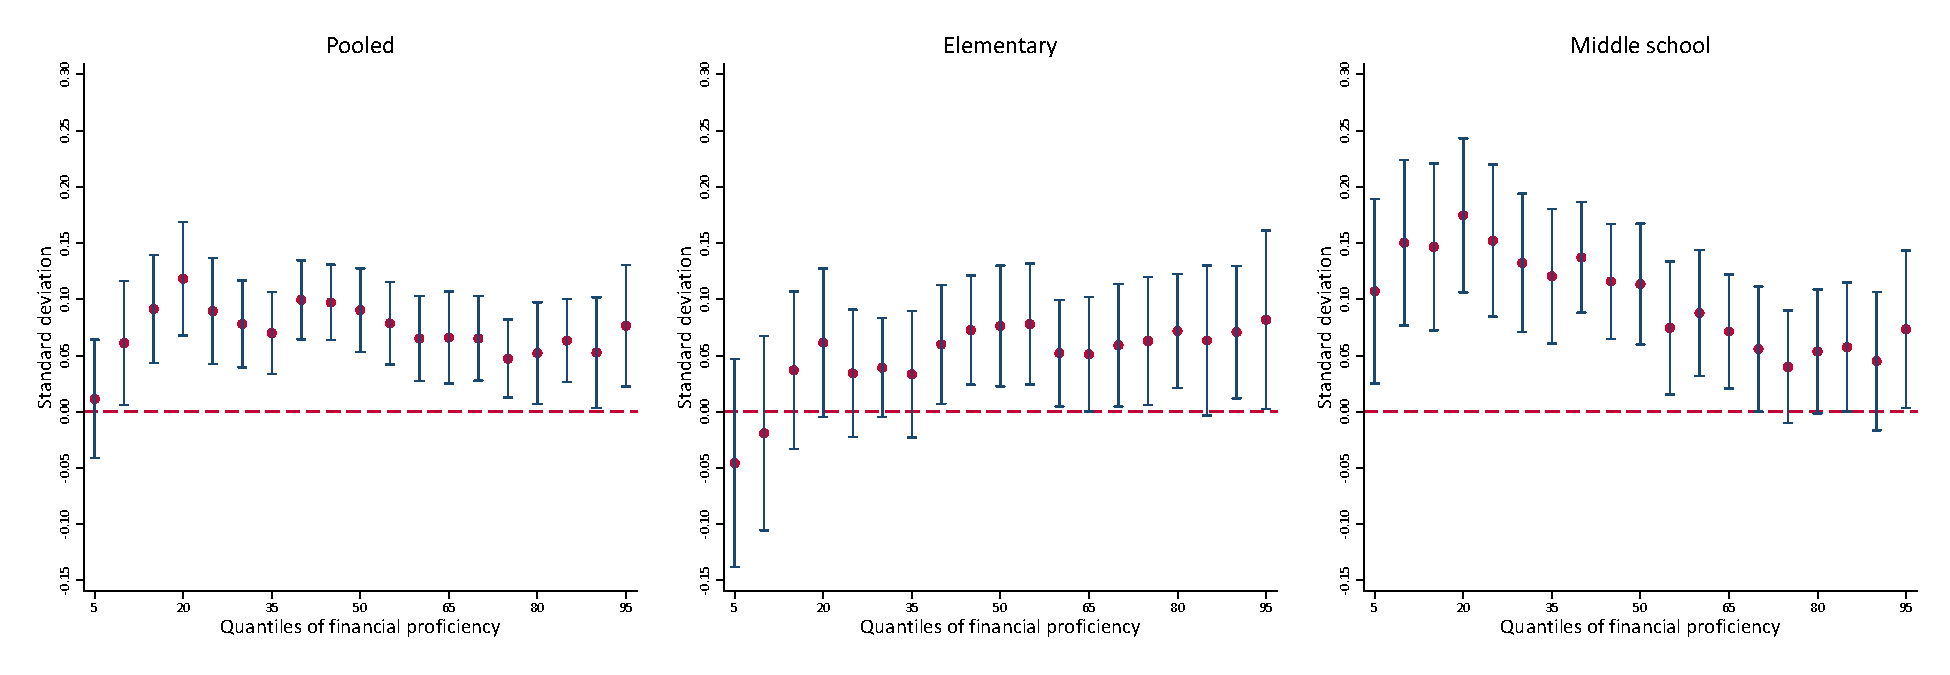
\includegraphics[width=\textwidth]{Figure2.pdf}
	    \label{fig:te_firstcycle}
     
     \raggedright
        \fontsize{9}{10} \selectfont

     {\textit{Note}: Financial proficiency is computed by CAEd from students' answers to a standardized test scored with Item Response Theory. The index is normalized to standard-deviation units, so treatment effects are read in standard deviations. We first run this financial proficiency score on the treatment dummy, the six strata dummies, and a constant. We then take the residuals from this estimation and run a simultaneous quantile regression for each quantile shown in the Figure, with the dependent variable being the residual from the first regression and the treatment dummy as the independent variable. 1000 bootstrap replications. The three panels report the pooled sample, elementary school students (third and fifth grades), and middle school students (seventh and ninth grades).}

     {\textit{Source}: Authors' estimates based on the pilot financial-literacy test applied by CAEd to students at the end of the 2015 school year.}
\end{figure}

\newpage

We further explore whether the program affected students' behavioral outcomes. These are self-reported measures, but more objective than the attitudional indeces. \autoref{tab:ITT_beha} shows that fifth graders are 5.7 pp (11.6 percent over the control mean) more likely to talk with their parents about money or family expenses, and 5.6 pp (28.4 percent) more likely to talk about money with their friends. Middle school students are also more likely to talk about money with their friends, but the effect size is small and statistically significant at 10 percent. 

Finally, we test whether the gains in financial proficiency and the more prudent attitudes toward saving and consumption, which might indicate that students became more forward-looking, translated into more investments in human capital. If that were the case, we would hypothesize lower repetition and dropout rates and a higher proficiency in Portuguese and/or math.

We look at grade repetition and dropout between 2015 and 2018; at \textit{Prova Brasil} Portuguese and math scores, measured in the pilot year for the fifth- and ninth-grade cohorts and two years later for the third- and seventh-grade cohorts; and, for the ninth-grade cohort, at high-school completion and \textit{ENEM} outcomes in 2018.

\autoref{tab:long-lasting} shows no systematic evidence that the program affected these outcomes. These outcomes are, however, observed over a relatively short window, one to three years after a low-intensity intervention, so changes that take longer to materialize, especially at these young ages, may fall outside what our data can capture.
 
\begin{table}[ht]
\centering
\begin{threeparttable}
\fontsize{9}{10}\selectfont
\caption{ITT estimates for human capital accumulation outcomes}\label{tab:long-lasting}
\begin{tabular*}{\textwidth}{@{\extracolsep{\fill}}l cccc}
\toprule
 & Third grade & Fifth grade & Seventh grade & Ninth grade \\
 & (1) & (2) & (3) & (4) \\
\midrule
\multicolumn{5}{l}{\textit{Panel A. Grade progression (School Census, cumulative 2015--2018)}} \\
{\bf Repetition} & 0.017 & 0.029** & -0.008 & 0.018 \\
  & (0.017) & (0.014) & (0.016) & (0.018) \\
{\bf Dropout} & 0.005 & 0.011 & 0.002 & 0.020 \\
  & (0.006) & (0.010) & (0.012) & (0.019) \\
\midrule
\multicolumn{5}{l}{\textit{Panel B. Test scores (\textit{Prova Brasil})}} \\
\textit{Assessed in} & \textit{2017} & \textit{2015} & \textit{2017} & \textit{2015} \\
{\bf Portuguese} & -0.029 & -0.017 & -0.005 & 0.028 \\
  & (0.047) & (0.046) & (0.034) & (0.036) \\
{\bf Math} & -0.066 & -0.033 & -0.009 & -0.020 \\
  & (0.053) & (0.049) & (0.038) & (0.039) \\
\midrule
\multicolumn{5}{l}{\textit{Panel C. End of high school (ninth-grade cohort assessed in 2018)}} \\
{\bf Graduated from high school} &  &  &  & -0.019 \\
  &  &  &  & (0.023) \\
{\bf Participated in ENEM} &  &  &  & -0.012 \\
  &  &  &  & (0.023) \\
{\bf Portuguese ENEM} &  &  &  & -0.025 \\
  &  &  &  & (0.031) \\
{\bf Math ENEM} &  &  &  & 0.002 \\
  &  &  &  & (0.045) \\
\midrule
Obs. & 4650 & 4755 & 3137 & 2851 \\
\bottomrule
\end{tabular*}
\begin{tablenotes}
\fontsize{9}{9}\selectfont
\item \textit{Notes}: Clustered standard errors at the school level in parentheses. Stars denote significance levels based on conventional p-values: * 10\%, ** 5\%, *** 1\%. The estimates were produced inside INEP's secure facility, where the bootstrap-based Romano-Wolf were not run; since the estimates are null, adjusting for multiple hypothesis testing would only reinforce the conclusions. Each dependent variable is regressed on treatment assignment, with one specification per cohort. Columns (1) and (2) include strata fixed effects only, since the third- and fifth-grade cohorts have no pre-pilot test score. Columns (3) and (4) add the student's pre-pilot fifth-grade \textit{Prova Brasil} performance, taken in 2013 by the seventh-grade cohort and in 2011 by the ninth-grade cohort, which controls for the pre-treatment imbalance documented in \autoref{tab:balance_adm2}.
\item \textit{Timing}: repetition and dropout (Panel A) are cumulative over 2015--2018. In Panel B, the ``Assessed in'' row gives the year each cohort sits \textit{Prova Brasil}: the fifth- and ninth-grade cohorts are assessed in the pilot year (2015, contemporaneous), while the third- and seventh-grade cohorts are assessed two years later (2017), when they reach the next assessment grade (see \autoref{tab:inep_data}). Panel C outcomes refer to 2018 and exist only for the ninth-grade cohort.
\item \textit{Source}: Authors' estimates based on the pilot roster merged with INEP's identified student-level administrative records (School Census, \textit{Prova Brasil}, and ENEM). INEP performed the merge; the authors ran all estimates inside INEP's secure facility.
\end{tablenotes}
\end{threeparttable}
\end{table}


Our estimates show that the program had larger impacts on financial proficiency in later grades and larger effects on attitudes and behavior in earlier grades. The results then suggest that the association between financial proficiency and behavioral change might not be straightforward. Individuals might have formal knowledge across different subjects, such as financial proficiency, but the application of that knowledge in real life can be hindered by the institutional environment they are embedded in \citep{carpena2020causal}. To formally test the hypothesis that learning mediates change in behavior, we follow \cite{imai2011unpacking} and
decompose the treatment effect estimates into the average causal mediation effect (ACME) and
the average causal direct effect (ADE).\footnote {See the online appendix for a formal discussion of Causal Mediation Effects.} The goal of this exercise is to assess the share of the change in behavioral outcomes that could be attributed to improvements in financial proficiency (ACME) and the share that comes directly from the program (ADE).\footnote{The decomposition of ITT effects on ACME and ADE relies on the sequential ignorability assumption. The first part of the assumption assumes that, conditioned on pre-treatment confounders, the treatment assignment is orthogonal to the potential outcomes and the mediator outcome (financial proficiency). The second part of the assumption implies that the observed mediator is ignorable given the actual treatment status and pre-treatment confounders \citep{imai2011unpacking}. This second part of the assumption is the strongest, even in the presence of random assignment. It posits that, conditional on the actual treatment (not the treatment assignment) and a vector of pre-treatment confounders, the outcome is independent of the mediator. Note that in our case, this implies the assumption that attitudinal and behavioral outcomes are orthogonal to financial proficiency, given the actual treatment and after controlling for a vector of school characteristics. Since we did not design the experiment to obtain clean estimates of the ACME and ADE, we interpret our results as suggestive evidence.}

\begin{table}[h!]
\centering
\begin{threeparttable}
\fontsize{9}{10}\selectfont
\caption{ITT estimates for behavioral outcomes}\label{tab:ITT_beha}
\begin{tabular*}{\textwidth}{@{\extracolsep{\fill}}l*{3}{c}}
\toprule
 & (1) & (2) & (3) \\
 & Pooled & Elementary & Middle school \\
\midrule
\tablefragment{../Datawork/Output/Tables/Table4.tex}
\bottomrule
\end{tabular*}
\begin{tablenotes}
\fontsize{9}{9}\selectfont
\item \textit{Notes}: Clustered standard errors at the school level in parentheses. RW denotes Romano-Wolf stepdown p-values (1{,}000 bootstrap replications resampling school clusters within randomization strata), adjusting for the joint testing of the 15 regressions reported in this table (every outcome in every subsample) as a single family, and RI denotes randomization inference (1{,}000 repetitions); both are reported below the standard error. Stars denote significance levels based on the Romano-Wolf adjusted p-value: * 10\%, ** 5\%, *** 1\%. Talking about money or expenses with parents equals 1 if the student reports discussing household expenses or talking about money with their parents, and 0 otherwise; the remaining variables equal 1 if the student talks about money with friends, keeps a piggy bank, has access to at least one financial service (bank account, debit card, or credit card), or receives an allowance from their parents, and 0 otherwise. The sample is restricted to fifth-, seventh-, and ninth-grade students.
\item \textit{Source}: Authors' estimates based on the pilot questionnaires applied by CAEd to students at the end of the 2015 school year.
\end{tablenotes}
\end{threeparttable}
\end{table}


According to the estimates in \autoref{tab:acme}, financial proficiency mediates part of the improvement in students' hypothetical attitudes toward consumption: among middle school students, the mediated component accounts for about half of the total effect. For elementary school students, by contrast, every mediated component is statistically indistinguishable from zero, so the effects on attitudes and on talking about money with parents and friends are direct. The same holds for the behavioral outcomes at both school levels, where the mediated components are negligible. In other words, the ADE and ACME estimates suggest that financial education programs affect students' attitudes and behavior through pathways other than the accumulation of formal knowledge. Overall, the estimates do not support the hypothesis that changes in financial proficiency are a necessary condition for changes in individuals' behavioral outcomes, a finding consistent with \citet{carpena2020causal} and \citet{de2021effect}.



\subsection{Robustness Check} 

As discussed in \autoref{sec:data_c}, the student-level merge with INEP's records recovers pre-treatment proficiency scores in reading and math for the seventh- and ninth-grade cohorts, and \autoref{tab:balance_adm2} shows that ninth-grade control students outperformed treated ones in reading before the pilot. Since principals, and not chance, chose the participating classes, this imbalance could bias our estimates. We therefore re-estimate \autoref{eq:Y} for these two cohorts controlling for their fifth-grade proficiency scores.\footnote{These are the only two cohorts with a pre-treatment performance score: seventh graders sat the fifth-grade test in 2013 and ninth graders in 2011.}

Controlling for past performance leads to a substantial gain in precision. Among ninth graders, the point estimate for financial proficiency rises from 0.107 to 0.149 of a standard deviation; and among seventh graders, it rises slightly from 0.09 to 0.098 (\autoref{tab:add_5prof_control}). The pattern suggests that ignoring the pre-treatment imbalance would underestimate the program's impact on financial proficiency, particularly for ninth graders. Controlling for past performance does not change the estimates for consumption and saving attitudes. 


\subsection{Implementation and IV Results}

As discussed in \autoref{sec:implementation}, we found evidence of contamination, especially in the control group. Because exposure to financial education content varied across classes within schools in both arms, the ITT compares assignment rather than exposure. To recover the effect of actual exposure, we use the random assignment as an instrument for exposure, following \cite{frisancho2023school}.

We measure exposure using two definitions, regardless of the arm to which the school was assigned. The conservative one is defined at the class level: it sets $Z=1$ when a teacher reports delivering financial education classes.\footnote{If the teacher answered the question ``\textit{How many financial education classes did you teach?}'', with answer categories running from one to eight or more, or the question ``\textit{What share of the student textbook did you cover?}'', with categories running from below 40\% to above 80\%.} For the classes whose teachers did not answer the teacher questionnaire, we set $Z=1$ if more than half of the students from those classes report having had such classes. The broad one is defined at the student level: it sets $Z=1$ when a teacher of the student's class reports delivering the financial education classes, as in the conservative definition, or when the student themselves reports having had them. Under the conservative definition, 97.8\% of students in treated classes and 11.1\% in control classes are classified as exposed; under the broad definition, 97.3\% and 21.5\%, respectively.

We estimate the local average treatment effect (LATE) by two-stage least squares. The first stage is
\begin{align}
     Z_{ism} = \pi_0 + \pi_1 T_{ism} + \sum_{n=1}^{6} \gamma_n + \nu_{ism}
     \label{eq:Y2}
\end{align}
and the second stage is
\begin{align}
    Y_{ism} = \lambda_0 + \lambda_1 \widehat{Z}_{ism} + \sum_{n=1}^{6} \gamma_n + \omega_{ism}
    \label{eq:Y3}
\end{align}
\noindent
where $Z$ is the exposure of student $i$'s class under the conservative definition and the student's own exposure under the broad one, $T$ is the random assignment of \autoref{eq:Y}, and the remaining notation follows that equation. Standard errors are clustered at the school level, the randomization unit. The parameter of interest, $\lambda_1$, is the LATE: the average effect of exposure among compliers, that is, the classes (under the conservative definition) or students (under the broad definition) that were exposed to the program because their school was assigned to the treatment group, and would not have been exposed otherwise.

\autoref{tab:iv} reports the LATE estimates next to the ITT under both definitions of exposure.\footnote{The first-stage estimates behind each LATE are reported in \autoref{tab:first_stage}.} For financial proficiency the differences are moderate: among middle school students, the effect rises from 0.099 of a standard deviation to 0.112 under the conservative definition and 0.135 under the broad one. For the attitude indices in grade 5, the correction is substantial: under the broad definition, the effect on the consumption index rises from 0.122 to 0.202 of a standard deviation, and on the saving index from 0.087 to 0.143. Exposure to the program therefore had modest effects on financial proficiency even among the classes that delivered the content, while its effects on the reported attitudes of younger students are sizeable once imperfect compliance is taken into account; since the broad definition relies on students' own reports, these larger estimates are best read as upper bounds.

\vspace{10 pt}

\begin{table}[h!]
\centering
\begin{threeparttable}
\fontsize{9}{10}\selectfont
\caption{Intention-to-treat (ITT) and local average treatment effect (LATE) estimates}\label{tab:iv}
\setlength{\tabcolsep}{2.5pt}
\begin{tabular*}{\textwidth}{@{\extracolsep{\fill}}l*{9}{c}}
\toprule
 & \multicolumn{3}{c}{Pooled} & \multicolumn{3}{c}{Elementary} & \multicolumn{3}{c}{Middle school} \\
\cmidrule(lr){2-4}\cmidrule(lr){5-7}\cmidrule(lr){8-10}
 & ITT & \shortstack{LATE\\ (i)} & \shortstack{LATE\\ (ii)} & ITT & \shortstack{LATE\\ (i)} & \shortstack{LATE\\ (ii)} & ITT & \shortstack{LATE\\ (i)} & \shortstack{LATE\\ (ii)} \\
\midrule
\tablefragment{../Datawork/Output/Tables/Table6.tex}
\bottomrule
\end{tabular*}
\begin{tablenotes}
\fontsize{9}{9}\selectfont
\item \textit{Notes}: Clustered standard errors at the school level in parentheses. RW denotes Romano-Wolf stepdown p-values (1{,}000 bootstrap replications resampling school clusters within randomization strata), adjusting for the joint testing of the 27 regressions reported in this table (every outcome, subsample, and estimator) as a single family, reported below the standard error. Stars denote significance levels based on the Romano-Wolf adjusted p-value: * 10\%, ** 5\%, *** 1\%. ITT is the reduced-form effect of random assignment; LATE instruments actual program exposure (\(Z\)) with random assignment. Exposure is measured under two definitions: (i) the conservative one, defined at the class level, which requires a teacher of the class to report having taught the financial education classes or covered part of the textbook, and, for the classes whose teachers did not answer their pilot questionnaire, that more than half of the students report having had such classes; and (ii) the broad one, defined at the student level, which sets \(Z=1\) when a teacher of the class reports delivering the classes or the student themselves reports having had them. Both are defined in the text. All three indices are normalized to standard-deviation units. The consumption and savings indices are unavailable for third graders, who did not answer these items. Therefore, elementary estimates represent the fifth grade, while middle school estimates represent the seventh and ninth grades. 
\item \textit{Source}: Authors' estimates based on the pilot questionnaires applied by CAEd to students at the end of the 2015 school year.
\end{tablenotes}
\end{threeparttable}
\end{table}

\clearpage
\input{06_conclusion}
\newpage


\bibliography{referencesp1}
\appendix

\counterwithin{table}{section}
\section{Tables}



% ==== Appendix tables, ordered by first citation (auto-reordered) ===
% Table A.1 -- shell for the fragment written by 2_Descriptives.do (figures from the World Bank's August 2016 report)
\begin{table}[htbp]
\centering
\fontsize{10}{11}\selectfont
\begin{threeparttable}
\caption{Sample selected for the pilot study}\label{tab:sample}
\begin{tabular*}{\textwidth}{@{\extracolsep{\fill}}lccccccc@{}}
\toprule
 & \multicolumn{3}{c}{Joinville} & \multicolumn{3}{c}{Manaus} & \\
\cmidrule(lr){2-4}\cmidrule(lr){5-7}
 & A.1 & A.2 & A.3 & B.1 & B.2 & B.3 & Total \\
Grades offered & 1--5 & 6--9 & 1--9 & 1--5 & 6--9 & 1--9 & \\
\midrule
\tablefragment{../Datawork/Output/Tables/TableA1.tex}
\bottomrule
\end{tabular*}
\begin{tablenotes}
\fontsize{9}{9}\selectfont
\item \textit{Notes}: Each column is one of the six strata, defined by municipality and school type. Row (1) is the sampling frame: 374 municipal schools offering elementary or middle school grades, 72 in Joinville and 302 in Manaus. Relative to the 2015 School Census, which records 369 municipal schools offering elementary and middle school education in Manaus and 83 in Joinville, the frame leaves out 67 schools in Manaus and 11 in Joinville. In Manaus, the majority of the schools out of the sample frame are in riverside communities that are very challenging to access for data collection. In Joinville, the 11 schools left out are all small rural schools. The 72 schools in the Joinville frame entered the study, as did all 65 Manaus schools offering grades 1--9 (stratum B.3). In strata B.1 and B.2, the budget did not allow us to survey every school, so we ranked schools by their 2013 IDEB, a school-level index that combines student performance in reading and mathematics with grade promotion rates, measured in grade 5 for the elementary grades and in grade 9 for the middle school grades, and drew the same number of schools at random from each quartile of that ranking, as shown in row (2). Within each of the six strata, we then randomly assigned roughly half of the schools to treatment and half to control, independently of the IDEB ranking; stratum B.3 holds an odd number of schools, hence 33 treated and 32 control.
\item \textit{Source}: Sampling frame from the pilot's implementation report, prepared by the World Bank in August 2016; school counts for the comparison with the census from the 2015 School Census (INEP). 
\end{tablenotes}
\end{threeparttable}
\end{table}

% TableA2 -- shell for the fragment written by 2_Descriptives.do
\begin{table}[ht]
\centering
\begin{threeparttable}
\fontsize{8}{10}\selectfont
\setlength{\tabcolsep}{3.5pt}
\caption{Program implementation, 2015}\label{tab:implementation}
\begin{tabular*}{\textwidth}{@{\extracolsep{\fill}}l*{9}{c}@{}}
\toprule
 & \multicolumn{3}{c}{Pooled} & \multicolumn{3}{c}{Elementary} & \multicolumn{3}{c}{Middle} \\
\cmidrule(lr){2-4}\cmidrule(lr){5-7}\cmidrule(lr){8-10}
 & C & T & Diff & C & T & Diff & C & T & Diff \\
\midrule
\tablefragment{../Datawork/Output/Tables/TableA2.tex}
\bottomrule
\end{tabular*}
\begin{tablenotes}
\fontsize{8}{10}\selectfont
\item \textit{Notes}: C and T are control and treatment means and Diff is the difference between them. Significance is from a regression of the indicator on treatment status and the strata dummies, with standard errors clustered at the school level: *** \(p<0.01\), ** \(p<0.05\), * \(p<0.1\). In Panel A, the unit of observation is the student in grades 5, 7, or 9, for which the data are available: Elementary is grade 5 and Middle is grades 7 and 9. In Panel B, the unit of observation is the teacher in charge of a pilot class: Elementary covers grades 3 and 5, and Middle grades 7 and 9.
\item \textit{Source}: Authors' estimates based on the pilot questionnaires applied by CAEd to students and teachers at the end of the 2015 school year.
\end{tablenotes}
\end{threeparttable}
\end{table}

\begin{table}[h!]
  \centering
\begin{threeparttable}
  \fontsize{8}{11}\selectfont
  \caption{Descriptors and skills on the financial knowledge test}\label{tab:descriptors}
    \begin{tabular}{lp{30.93em}cccc}
    \toprule
 & \multicolumn{1}{r}{} & Third grade & Fifth grade    & Seventh grade  & Ninth grade  \\
    \midrule
    D01   & Being able to identify the subject of texts whose topic explores socially responsible attitudes towards the environment  & yes   & yes   & yes   & yes \\
    D02   & Being able to find information in texts about consumption – light, water, telephone bills, among others  & yes   & yes   & no    & no \\
    D03   & Being able to identify the purpose of texts and text formats that include expenses, consumption, spending  & yes   & yes   & no    & no \\
    D04   & Being able to recognize the purpose of text genres related to finances – receipts, checks, invoices & no    & yes   & yes   & yes \\
    D05   & Being able to recognize situations in which concepts related to finances are present: savings, expenses, consumption, spending, waste, risk, return, financial planning, and investment, among others.  & no    & no    & yes   & yes \\
    D06   & Being able to identify situations related to financially responsible attitudes  & no    & yes   & yes   & yes \\
    D07   & Being able to find information in graphs and tables that contain data related to finances (purchases, sales, spending) & yes   & no    & no    & no \\
    D08   & Being able to find information in texts that circulate in the financial world: classified ads, news features, among others & yes   & yes   & yes   & yes \\
    D09   & Being able to estimate values and/or procedures necessary for financial projects & yes   & yes   & yes   & yes \\
    D10   & Being able to distinguish remunerated from non-remunerated work. & yes   & yes   & no    & no \\
    D11   & Being able to identify the origin and destination of varied products and/or those that can be recycled. & yes   & no    & no    & no \\
    D12   & Being able to recognize socially responsible situations related to public and private spaces. & no    & no    & no    & yes \\
    D13   & Being able to identify advantages, disadvantages, and risks of cash and credit sales. & no    & yes   & no    & yes \\
    D14   & Being able to find implicit information in media texts that are relevant for decision-making in finances.  & no    & yes   & yes   & yes \\
    \bottomrule
    \end{tabular}%
\begin{tablenotes}
\fontsize{8}{9}\selectfont
\item \textit{Notes}: Each row is a skill descriptor assessed by the financial literacy test; ``yes'' indicates the descriptor is assessed in that grade. The test content is adapted to each grade, so not every descriptor appears in every grade.
\item \textit{Source}: Authors' elaboration based on the financial literacy test applied by CAEd at the end of the 2015 school year.
\end{tablenotes}
\end{threeparttable}
\end{table}%

\begin{table}[h!]
  \centering
  \fontsize{8}{10} \selectfont
\begin{threeparttable}
  \caption{Items used to construct the consumption and savings attitude indices}\label{tab:cs_index}%
     \setlength{\tabcolsep}{4pt}%
     \begin{tabular}{p{7.4cm}ccccc}
    \textbf{Statement} & \multicolumn{4}{c}{\textbf{Answers' scale}} & \textbf{Weight} \\
    \midrule
          & Totally agree & Agree & Disagree & Totally disagree &  \\
\tablefragment{../Datawork/Output/Tables/TableA4.tex}
    \bottomrule
    \end{tabular}%
\begin{tablenotes}
\fontsize{8}{9}\selectfont
\item \textit{Notes}: The table lists every item used to build the two indices --- seven for consumption and eight for savings --- and not a selection of them. Each item was printed in the questionnaire as a statement, and students chose the option they most agreed with on a four-point scale. The figures under \textit{Answers' scale} show how each option was coded: because the statements are worded in both directions, the coding is reversed for the positively worded items so that 4 always corresponds to the most prudent response.

\item Each index is the first principal component of the items in its block, standardized to mean zero and unit variance. \textit{Weight} reports the loading the principal component places on each item; the loadings are estimated from the correlation between items across students and are normalized so that their squares sum to one within each block. The first component accounts for 36.6\% of the variation across the consumption items and 34.5\% across the savings items.

\item The attitudes questionnaire was administered only in grades 5, 7, and 9; the statements were not part of the third-grade questionnaire, so neither index is available for that grade. Of the 11,020 students in grades 5, 7, and 9 who took the financial literacy test, 10,823 (98\%) also completed the attitudes questionnaire. Each index requires the full block of items: the consumption index is computed for the 10,220 students who answered all seven consumption statements, and the savings index for the 10,022 who answered all eight savings statements. A student who skipped any statement in a block, or who did not complete the questionnaire, has no index for that block.
\item \textit{Source}: Authors' elaboration based on the pilot student questionnaire applied by CAEd at the end of the 2015 school year.
\end{tablenotes}
\end{threeparttable}
\end{table}%

\newgeometry{left=1.5cm, right=1.5cm, top=2cm, bottom=2cm}
% TableA5 -- shell for the fragment written by 2_Descriptives.do
\begin{table}[ht]
\centering
\begin{threeparttable}
\fontsize{7}{8}\selectfont
\setlength{\tabcolsep}{2.5pt}
\caption{Balance test for students}\label{tab:studentscar}
\begin{tabular*}{\textwidth}{@{\extracolsep{\fill}}p{3.1cm}l*{12}{c}@{}}
\toprule
 & & \multicolumn{3}{c}{Third grade} & \multicolumn{3}{c}{Fifth grade} & \multicolumn{3}{c}{Seventh grade} & \multicolumn{3}{c}{Ninth grade} \\
\cmidrule(lr){3-5}\cmidrule(lr){6-8}\cmidrule(lr){9-11}\cmidrule(lr){12-14}
 & & C & T & Diff & C & T & Diff & C & T & Diff & C & T & Diff \\
\midrule
\tablefragment{../Datawork/Output/Tables/TableA5.tex}
\bottomrule
\end{tabular*}
\begin{tablenotes}
\fontsize{7}{8}\selectfont
\item \textit{Notes}: C = control, T = treatment; Diff is the difference between the two group means. Means and differences are in percentage points, with the standard error of each mean in parentheses. Balance is computed one variable at a time with \texttt{iebaltab}, taking the randomization strata as covariates and clustering standard errors at the school level; stars are from that test: *** \(p<0.01\), ** \(p<0.05\), * \(p<0.1\). The first two rows report participation in the financial literacy assessment and, among participants, the response rate to the socioeconomic questionnaire, answered by the legal guardians in the third grade.
\item \textit{Source}: Authors' estimates based on the pilot socioeconomic questionnaire applied by CAEd at the end of the 2015 school year.
\end{tablenotes}
\end{threeparttable}
\end{table}
\restoregeometry

\newgeometry{left=1.5cm, right=1.5cm, top=2cm, bottom=2cm}
% TableA6 -- shell for the fragment written by 2_Descriptives.do
\begin{table}[ht]
\centering
\begin{threeparttable}
\fontsize{7}{8}\selectfont
\setlength{\tabcolsep}{2.5pt}
\caption{Balance test for teachers}\label{tab:teacherscar}
\begin{tabular*}{\textwidth}{@{\extracolsep{\fill}}p{3.1cm}l*{12}{c}@{}}
\toprule
 & & \multicolumn{3}{c}{Third grade} & \multicolumn{3}{c}{Fifth grade} & \multicolumn{3}{c}{Seventh grade} & \multicolumn{3}{c}{Ninth grade} \\
\cmidrule(lr){3-5}\cmidrule(lr){6-8}\cmidrule(lr){9-11}\cmidrule(lr){12-14}
 & & C & T & Diff & C & T & Diff & C & T & Diff & C & T & Diff \\
\midrule
\tablefragment{../Datawork/Output/Tables/TableA6.tex}
\bottomrule
\end{tabular*}
\begin{tablenotes}
\fontsize{7}{8}\selectfont
\item \textit{Notes}: C = control, T = treatment; Diff is the difference between the two group means. Means and differences are in percentage points, with the standard error of each mean in parentheses. Balance is computed one variable at a time with \texttt{iebaltab}, taking the randomization strata as covariates and clustering standard errors at the school level; stars are from that test: *** \(p<0.01\), ** \(p<0.05\), * \(p<0.1\).
\item \textit{Source}: Authors' estimates based on the pilot teacher questionnaire applied by CAEd at the end of the 2015 school year.
\end{tablenotes}
\end{threeparttable}
\end{table}
\restoregeometry

\newgeometry{left=2cm, right=2cm, top=1cm, bottom=1cm}
% TableA7 -- shell for the fragment written by 2_Descriptives.do
\begin{table}[htbp]
\centering
\begin{threeparttable}
\fontsize{8}{8}\selectfont
\caption{Pre-treatment balance test with administrative data at school level}\label{tab:pret_balancing}
\begin{tabular*}{\textwidth}{@{\extracolsep{\fill}}p{20em}ccccc@{}}
\toprule
 & \multicolumn{2}{c}{(1) Control} & \multicolumn{2}{c}{(2) Treatment} & T-Test \\
\cmidrule(lr){2-3}\cmidrule(lr){4-5}
 & N & Mean/SE & N & Mean/SE & Difference (1)-(2) \\
\midrule
\tablefragment{../Datawork/Output/Tables/TableA7.tex}
\bottomrule
\end{tabular*}
\begin{tablenotes}
\fontsize{9}{9}\selectfont
\item \textit{Notes}: Columns (1) and (2) report the control and treatment group means, with the standard error of each mean in parentheses; N is the number of schools. The difference column reports the control-minus-treatment difference between the two group means. Significance is from a regression of the covariate on treatment status and the six strata dummies, with standard errors clustered at the randomization-group level: *** \(p<0.01\), ** \(p<0.05\), * \(p<0.1\). Covariates are drawn from public administrative records (School Census, \textit{Prova Brasil}, and IDEB) for the years shown.
\item \textit{Source}: Authors' estimates based on public school-level administrative records from INEP (School Census, \textit{Prova Brasil}, and IDEB).
\end{tablenotes}
\end{threeparttable}
\end{table}
\restoregeometry

\newgeometry{left=2cm, right=2cm, top=1.2cm, bottom=1.2cm}
\begin{table}[h!]
  \centering
  \begin{threeparttable}
  \fontsize{9}{10}\selectfont
  \caption{Pre-treatment balance test for third and fifth graders}\label{tab:balance_adm1}
\begin{tabular*}{\textwidth}{@{\extracolsep{\fill}}lccccc@{}}
\toprule
           & \multicolumn{ 2}{c}{(1)} & \multicolumn{ 2}{c}{(2)} &     T-Test \\

           & \multicolumn{ 2}{c}{Control} & \multicolumn{ 2}{c}{Treament} & Difference \\

           &          N &    Mean/SE &          N &    Mean/SE &    (1)-(2) \\
\midrule
{\it {\bf Third grade}} &            &            &            &            &            \\

Beneficiary of Bolsa Família &       1082 &      36.23 &       1059 &      36.07 &       0.16 \\

           &            &     (3.10) &            &     (2.92) &            \\

Adequate age for their grade &       1038 &      86.99 &        997 &      85.66 &       1.34 \\

           &            &     (1.49) &            &     (1.76) &            \\

Gender: male &       2071 &      53.84 &       2009 &      51.57 &       2.27 \\

           &            &     (0.92) &            &     (1.22) &            \\

Color: white &       1624 &      38.92 &       1582 &      36.47 &       2.44 \\

           &            &     (3.80) &            &     (3.94) &            \\

Mother education/Legal guardian: at least high school degree &       1081 &      53.01 &       1050 &      50.95 &       2.05 \\

           &            &     (2.59) &            &     (2.26) &            \\

Student found in School Census 2015-2018 &       2380 &      87.02 &       2270 &      88.50 &      -1.49 \\

           &            &     (1.60) &            &     (1.51) &            \\

Student found in Prova Brasil 2017 &       2380 &      59.03 &       2270 &      59.16 &      -0.13 \\

           &            &     (1.84) &            &     (1.89) &            \\

Prova Brasil reading score in 5th grade 2017 &       1405 &     232.76 &       1343 &     230.43 &       2.33 \\

           &            &     (2.51) &            &     (2.45) &            \\

Prova Brasil math score in 5th grade 2017 &       1405 &     243.09 &       1343 &     238.55 &       4.54 \\

           &            &     (2.92) &            &     (3.09) &            \\

{\it {\bf Fifth grade}} &            &            &            &            &            \\

Beneficiary of Bolsa Família &       1905 &      45.35 &       1958 &      44.94 &       0.41 \\

           &            &     (2.80) &            &     (2.65) &            \\

Adequate age for their grade &       1902 &      78.39 &       1952 &      77.61 &       0.78 \\

           &            &     (1.71) &            &     (1.58) &            \\

Gender: male &       2302 &      51.87 &       2307 &      50.59 &       1.28 \\

           &            &     (1.12) &            &     (1.10) &            \\

Color: white &       1888 &      40.57 &       1945 &      37.33 &       3.25 \\

           &            &     (2.52) &            &     (2.48) &            \\

Mother education/Legal guardian: at least high school degree &       1272 &      55.66 &       1333 &      56.04 &      -0.38 \\

           &            &     (1.87) &            &     (2.00) &            \\

Student found in School Census 2015-2018 &       2375 &      89.94 &       2380 &      90.04 &      -0.11 \\

           &            &     (1.52) &            &     (1.08) &            \\

Student found in Prova Brasil 2015 &       2375 &      79.33 &       2380 &      81.60 &      -2.27 \\

           &            &     (2.22) &            &     (1.77) &            \\

Prova Brasil reading score in 5th grade 2017 &       1884 &     220.58 &       1942 &     218.95 &       1.62 \\

           &            &     (2.92) &            &     (2.68) &            \\

Prova Brasil math score in 5th grade 2017 &       1884 &     231.83 &       1942 &     229.17 &       2.66 \\

           &            &     (3.82) &            &     (3.33) &            \\

           &            &            &            &            &            \\


\bottomrule
\end{tabular*}
\begin{tablenotes}
\fontsize{9}{9}\selectfont
\item \textit{Notes}: We run the balance test controlling for strata. All variables are from \textit{Prova Brasil} and the School Census. *** $p<0.01$, ** $p<0.05$, * $p<0.1$.
\item \textit{Source}: Authors' estimates based on the pilot roster merged with INEP's identified student-level administrative records (\textit{Prova Brasil} and School Census); INEP performed the merge and the authors ran all balance tests inside INEP's secure facility.
\end{tablenotes}
\end{threeparttable}
\end{table}
\restoregeometry

\newgeometry{left=2cm, right=2cm, top=1.2cm, bottom=1.2cm}
\begin{table}[h!]
  \centering
  \begin{threeparttable}
  \fontsize{9}{10}\selectfont
  \caption{Pre-treatment balance test for seventh and ninth graders}\label{tab:balance_adm2}
\begin{tabular*}{\textwidth}{@{\extracolsep{\fill}}lccccc@{}}
\toprule
           & \multicolumn{ 2}{c}{(1)} & \multicolumn{ 2}{c}{(2)} &     T-Test \\

           & \multicolumn{ 2}{c}{Control} & \multicolumn{ 2}{c}{Treament} & Difference \\

           &          N &    Mean/SE &          N &    Mean/SE &    (1)-(2) \\
\midrule
{\it {\bf Seventh grade}} &            &            &            &            &            \\

Beneficiary of Bolsa Família &       1790 &      40.95 &       1788 &      42.90 &      -1.95 \\

           &            &     (2.92) &            &     (2.87) &            \\

Adequate age for their grade &       1781 &      77.20 &       1781 &      76.81 &       0.39 \\

           &            &     (2.18) &            &     (1.85) &            \\

Gender: male &       1798 &      48.00 &       1799 &      48.08 &      -0.08 \\

           &            &     (1.45) &            &     (1.04) &            \\

Color: white &       2226 &      31.63 &       2186 &      32.20 &      -0.58 \\

           &            &     (4.09) &            &     (3.89) &            \\

Mother education/Legal guardian: at least high school degree &       1347 &      52.64 &       1317 &      54.75 &      -2.11 \\

           &            &     (2.01) &            &     (2.05) &            \\

Student found in School Census 2015-2018 &       2376 &      91.20 &       2321 &      91.12 &       0.08 \\

           &            &     (1.66) &            &     (1.11) &            \\

Student found in Prova Brasil 2013 &       2376 &      67.05 &       2321 &      66.52 &       0.52 \\

           &            &     (2.25) &            &     (1.91) &            \\

Prova Brasil reading score in 5th grade 2013 &       1593 &     211.03 &       1544 &     209.28 &       1.75 \\

           &            &     (3.16) &            &     (2.68) &            \\

Prova Brasil math score in 5th grade 2013 &       1593 &     226.11 &       1544 &     224.70 &       1.41 \\

           &            &     (4.10) &            &     (3.66) &            \\

Student found in Prova Brasil 2017 &       2376 &      62.50 &       2321 &      61.83 &       0.67 \\

           &            &     (2.04) &            &     (1.88) &            \\

Prova Brasil reading score in 9th grade 2017 &       1485 &     273.81 &       1435 &     274.74 &      -0.93 \\

           &            &     (2.58) &            &     (2.31) &            \\

Prova Brasil math score in 9th grade 2017 &       1485 &     269.66 &       1435 &     271.07 &      -1.42 \\

           &            &     (3.48) &            &     (3.01) &            \\

{\it {\bf Ninth grade}} &            &            &            &            &            \\

Beneficiary of Bolsa Família &       1648 &      38.35 &       1604 &      35.79 &      2.56* \\

           &            &     (3.07) &            &     (2.59) &            \\

Adequate age for their grade &       1636 &      76.96 &       1602 &      76.09 &       0.86 \\

           &            &     (1.80) &            &     (2.30) &            \\

Gender: male &       2161 &      49.56 &       2174 &      47.10 &      2.46* \\

           &            &     (1.05) &            &     (1.08) &            \\

Color: white &       2074 &      32.64 &       2087 &      30.09 &       2.55 \\

           &            &     (4.22) &            &     (3.95) &            \\

Mother education/Legal guardian: at least high school degree &       1364 &      57.26 &       1335 &      57.00 &       0.25 \\

           &            &     (1.75) &            &     (1.77) &            \\

Student found in School Census 2015-2018 &       2222 &      92.26 &       2233 &      92.79 &      -0.53 \\

           &            &     (0.98) &            &     (0.84) &            \\

Student found in Prova Brasil 2011 &       2222 &      63.77 &       2233 &      64.22 &      -0.45 \\

           &       (72) &     (2.24) &       (72) &     (2.06) &            \\

Prova Brasil reading score in 5th grade 2011 &       1417 &     206.10 &       1434 &     200.39 &     5.71** \\

           &       (71) &     (3.07) &       (72) &     (2.78) &            \\

Prova Brasil math score in 5th grade 2011 &       1417 &     221.42 &       1434 &     215.72 &       5.69 \\

           &       (71) &     (3.80) &       (72) &     (3.59) &            \\

Student found in Prova Brasil 2015 &       2222 &      82.36 &       2233 &      81.10 &       1.26 \\

           &       (72) &     (1.31) &       (72) &     (1.45) &            \\

Prova Brasil reading score in 9th grade 2015 &       1830 &     265.01 &       1811 &     264.14 &       0.87 \\

           &       (70) &     (2.27) &       (70) &     (1.92) &            \\

Prova Brasil math score in 9th grade 2015 &       1830 &     264.88 &       1811 &     260.73 &      4.15* \\

           &       (70) &     (2.73) &       (70) &     (2.74) &            \\

Graduated from high school &       2222 &      59.63 &       2233 &      56.02 &       3.61 \\

           &       (72) &     (1.58) &       (72) &     (1.91) &            \\

Participated in ENEM, 2018 &       2222 &      46.17 &       2233 &      43.62 &       2.56 \\

           &       (72) &     (1.54) &       (72) &     (1.83) &            \\

Standardized ENEM score, 2018 &        793 &       0.13 &        723 &       0.12 &       0.01 \\

           &       (71) &     (0.04) &       (71) &     (0.05) &            \\

           &            &            &            &            &            \\

\bottomrule
\end{tabular*}
\begin{tablenotes}
\fontsize{9}{9}\selectfont
\item \textit{Notes}: We run the balance test controlling for strata. All variables are from \textit{Prova Brasil} and the School Census. *** $p<0.01$, ** $p<0.05$, * $p<0.1$.
\item \textit{Source}: Authors' estimates based on the pilot roster merged with INEP's identified student-level administrative records (\textit{Prova Brasil} and School Census); INEP performed the merge and the authors ran all balance tests inside INEP's secure facility.
\end{tablenotes}
\end{threeparttable}
\end{table}
\restoregeometry

\begin{landscape}
\begin{table}[htbp]
\centering
\begin{threeparttable}
\fontsize{7}{9}\selectfont
\caption{Average causal mediation effects (mediator: financial proficiency)}\label{tab:acme}
\setlength{\tabcolsep}{3pt}
\begin{tabular*}{\textwidth}{@{\extracolsep{\fill}}l*{7}{cc}@{}}
\toprule
  & \multicolumn{2}{c}{Consumption} & \multicolumn{2}{c}{Saving} & \multicolumn{2}{c}{Talks with parents} & \multicolumn{2}{c}{Talks with friends} & \multicolumn{2}{c}{Piggy bank use} & \multicolumn{2}{c}{Use of financial services} & \multicolumn{2}{c}{Receiving an allowance} \\
\cmidrule(lr){2-3}\cmidrule(lr){4-5}\cmidrule(lr){6-7}\cmidrule(lr){8-9}\cmidrule(lr){10-11}\cmidrule(lr){12-13}\cmidrule(lr){14-15}
  & Mean & 95\% CI & Mean & 95\% CI & Mean & 95\% CI & Mean & 95\% CI & Mean & 95\% CI & Mean & 95\% CI & Mean & 95\% CI \\
\midrule
\tablefragment{../Datawork/Output/Tables/TableA10.tex}
\bottomrule
\end{tabular*}
\begin{tablenotes}
\fontsize{7}{8}\selectfont
\item \textit{Notes}: Each dependent variable equals 1 if the student talks to their parents or friends about financial subjects, keeps a piggy bank, has access to financial services, or receives an allowance, and 0 otherwise; consumption and savings are the standardized attitude indices. The mediator is the financial-proficiency index. \textit{Total effect} is the total treatment effect ($\tau$), \textit{ADE} the average direct effect, \textit{ACME} the average causal mediation effect operating through financial proficiency, and \textit{\% mediated} the share of the total effect that runs through the mediator. Estimated with the \texttt{medeff} command; 95\% confidence intervals in brackets from 1{,}000 simulations. Controls: strata, school infrastructure, and syllabus complexity. The sample is restricted to fifth-, seventh-, and ninth-grade students: third graders, who answered only the piggy-bank and financial-services items, are excluded so that all outcomes cover the same grades.
\item \textit{Source}: Authors' estimates based on the pilot questionnaires applied by CAEd to students at the end of the 2015 school year, merged with school-level administrative records.
\end{tablenotes}
\end{threeparttable}
\end{table}
\end{landscape}

\begin{table}[ht]
\centering
\begin{threeparttable}
\fontsize{9}{10}\selectfont
\caption{ITT estimates controlling for pre-pilot performance}\label{tab:add_5prof_control}
\begin{tabular*}{\textwidth}{@{\extracolsep{\fill}}lcccc@{}}
\toprule
 & \multicolumn{2}{c}{Seventh grade} & \multicolumn{2}{c}{Ninth grade} \\
\cmidrule(lr){2-3}\cmidrule(lr){4-5}
 & (1) & (2) & (3) & (4) \\
 & Strata FE & \shortstack{Strata FE +\\ pre-pilot performance} & Strata FE & \shortstack{Strata FE +\\ pre-pilot performance} \\
\midrule
\textbf{Financial proficiency} &  &  &  &  \\
Treatment   &     0.090* &    0.098** &     0.107* &   0.149*** \\
            &    (0.048) &    (0.042) &    (0.056) &    (0.055) \\
RI pvalue   &      0.061 &      0.022 &      0.057 &      0.008 \\
N. obs      &       3640 &       2538 &       3374 &       2251 \\
R-squared   &      0.208 &      0.505 &      0.168 &      0.399 \\
\midrule
\textbf{Consumption index} &  &  &  &  \\
Treatment   &     0.080* &     0.070* &    0.084** &     0.087* \\
            &    (0.041) &    (0.042) &    (0.037) &    (0.044) \\
RI pvalue   &      0.054 &      0.098 &      0.025 &      0.050 \\
N. obs      &       3409 &       2384 &       3163 &       2115 \\
R-squared   &      0.100 &      0.187 &      0.055 &      0.128 \\
\midrule
\textbf{Saving index} &  &  &  &  \\
Treatment   &      0.066 &      0.033 &      0.018 &      0.030 \\
            &    (0.040) &    (0.044) &    (0.038) &    (0.045) \\
RI pvalue   &      0.102 &      0.456 &      0.644 &      0.508 \\
N. obs      &       3368 &       2351 &       3105 &       2080 \\
R-squared   &      0.032 &      0.065 &      0.019 &      0.044 \\
\bottomrule
\end{tabular*}
\begin{tablenotes}
\fontsize{9}{9}\selectfont
\item \textit{Notes}: Clustered standard errors at the school level in parentheses; RI denotes randomization inference. *** $p<0.01$, ** $p<0.05$, * $p<0.1$. Columns (2) and (4) add the student's fifth-grade \textit{Prova Brasil} reading and math scores, taken in 2013 for the seventh-grade cohort and in 2011 for the ninth-grade cohort, as controls; the smaller sample in these columns reflects the students the merge with INEP's records located in those waves. Financial proficiency is computed by CAEd from students' answers to a standardized test scored with Item Response Theory. The consumption and savings indices summarize students' answers to fifteen agreement-scale statements, reported with their weights in \autoref{tab:cs_index}. All three indices are normalized to standard-deviation units, so treatment effects are read in standard deviations.
\item \textit{Source}: Authors' estimates based on the pilot roster merged with INEP's identified student-level administrative records (School Census and \textit{Prova Brasil}). INEP performed the merge; the authors ran all estimates inside INEP's secure facility.
\end{tablenotes}
\end{threeparttable}
\end{table}

\newgeometry{left = 2.54cm, right = 2.54cm, top = 2.5cm, bottom = 2.5cm}



\counterwithin{figure}{section}












\end{document}

%One way to read the figures is to by setting the ACME at zero. For the consumption and savings index, the sensitive parameter associated with ACME = 0 is around 0.5. This means that there should be an omitted bias accounting for 0.7 of the remaining variance in both the mediator and outcome equations (0.7 x 0.7 $\approx$ 0.5) which seems implausible. Very similar parameters are found when we split the analysis by school grades. However, the parameter is close to zero for the behavioral outcomes suggesting that the estimated results are very sensitive to omitted confounders. The ADE and ACME estimates should then be interpreted with caution given that the strong ignorability assumption may not hold in most estimates.  